%!TEX root = ../thesis.tex

\chapter{Infrastructure}
\label{sec:infrastructure}

The infrastructure implements a server-client design pattern and is divided into two parts:
The \emph{Server} part and the \emph{Local} part.
First, the server is an independent unit providing a public API to its clients.
Second, the local part is a client consuming the provided API to retrieve configuration from the server and populate it with data gathered from the deployed residential infrastructure.
Both parts will be explained in the following sections.

\section{Server Infrastructure}
\label{sec:server_infrastructure}

The server is the main storage and communication center of this project.
It persists data collected by the local deployment as also organizational information and heating schedules provided by the user via the Mobile App.

\subsection{Design Goals}

\begin{itemize}
\item \emph{Modularity} for independent, interchangeable components for improved Maintainability.
\item \emph{Extensibility} to easily add new resources and relationships.
\item \emph{Usability} for developers.
\item \emph{Testability} for good and comprehensible tests.
\end{itemize}

\subsection{Platform and Frameworks}

The server is implemented with Python, a general-purpose, multi-paradigm programming language\footnote{\url{https://www.python.org/}}.
Python was chosen as it is suitable for developing a solid web server as also for usage on restricted hardware like the Raspberry Pi used for the local deployment.
Django\footnote{\url{https://www.djangoproject.com/}} is a popular web application framework based on a model-view-controller (MVC) pattern facilitating the development of complex, database-driven web applications.
The Django REST Framework\footnote{\url{http://www.django-rest-framework.org/}} extends Django to support the design of RESTful Web APIs.

\subsection{RESTful API}

The server provides a RESTful API designed to persist temperature and heating schedule data of several thermostats.

Each resource is identified by a uniform resource identifier (URI). There are two major types of URIs, resource collections and resource representations.
A resource representation is a view of its resource's state and is usually encoded in XML or JSON.
Resource collections can contain multiple representations of the same type of a resource.

\paragraph{Design Decisions}

\begin{itemize}
    \itemsep0em
    \item Resource collections are referenced per URL. Resources are referenced by including their representation.
    \item URL fields are identified by the name \emph{url} or the suffix \emph{\_url}. Each resource representation contains its own URL in the field \emph{url}.
\end{itemize}

\paragraph{Browsable API}

The Django REST Framework 

Discoverability



\subsection{Program Architecture and Implementation}

The server implementation is built on the Django Framework following a variation\footnote{\url{https://docs.djangoproject.com/en/1.8/faq/general/\#django-appears-to-be-a-mvc-framework-but-you-call-the-controller-the-view-and-the-view-the-template-how-come-you-don-t-use-the-standard-names}} of the Model-View-Controller (MVC) architectural pattern\footnote{\url{https://en.wikipedia.org/wiki/Model-view-controller}}. We assume the user to be familiar with the common MVC pattern.\todo{Explain Djangos architecture?}

\subsubsection{Models}

Models provide an abstraction layer for structuring and manipulating data handled by the web application\todo[fancyline]{Rewrite this sentence, less copying.}.
% A high level description of all used models is given in Section~\ref{sec:system_overview_models}. 

\begin{figure}[h]
\begin{center}
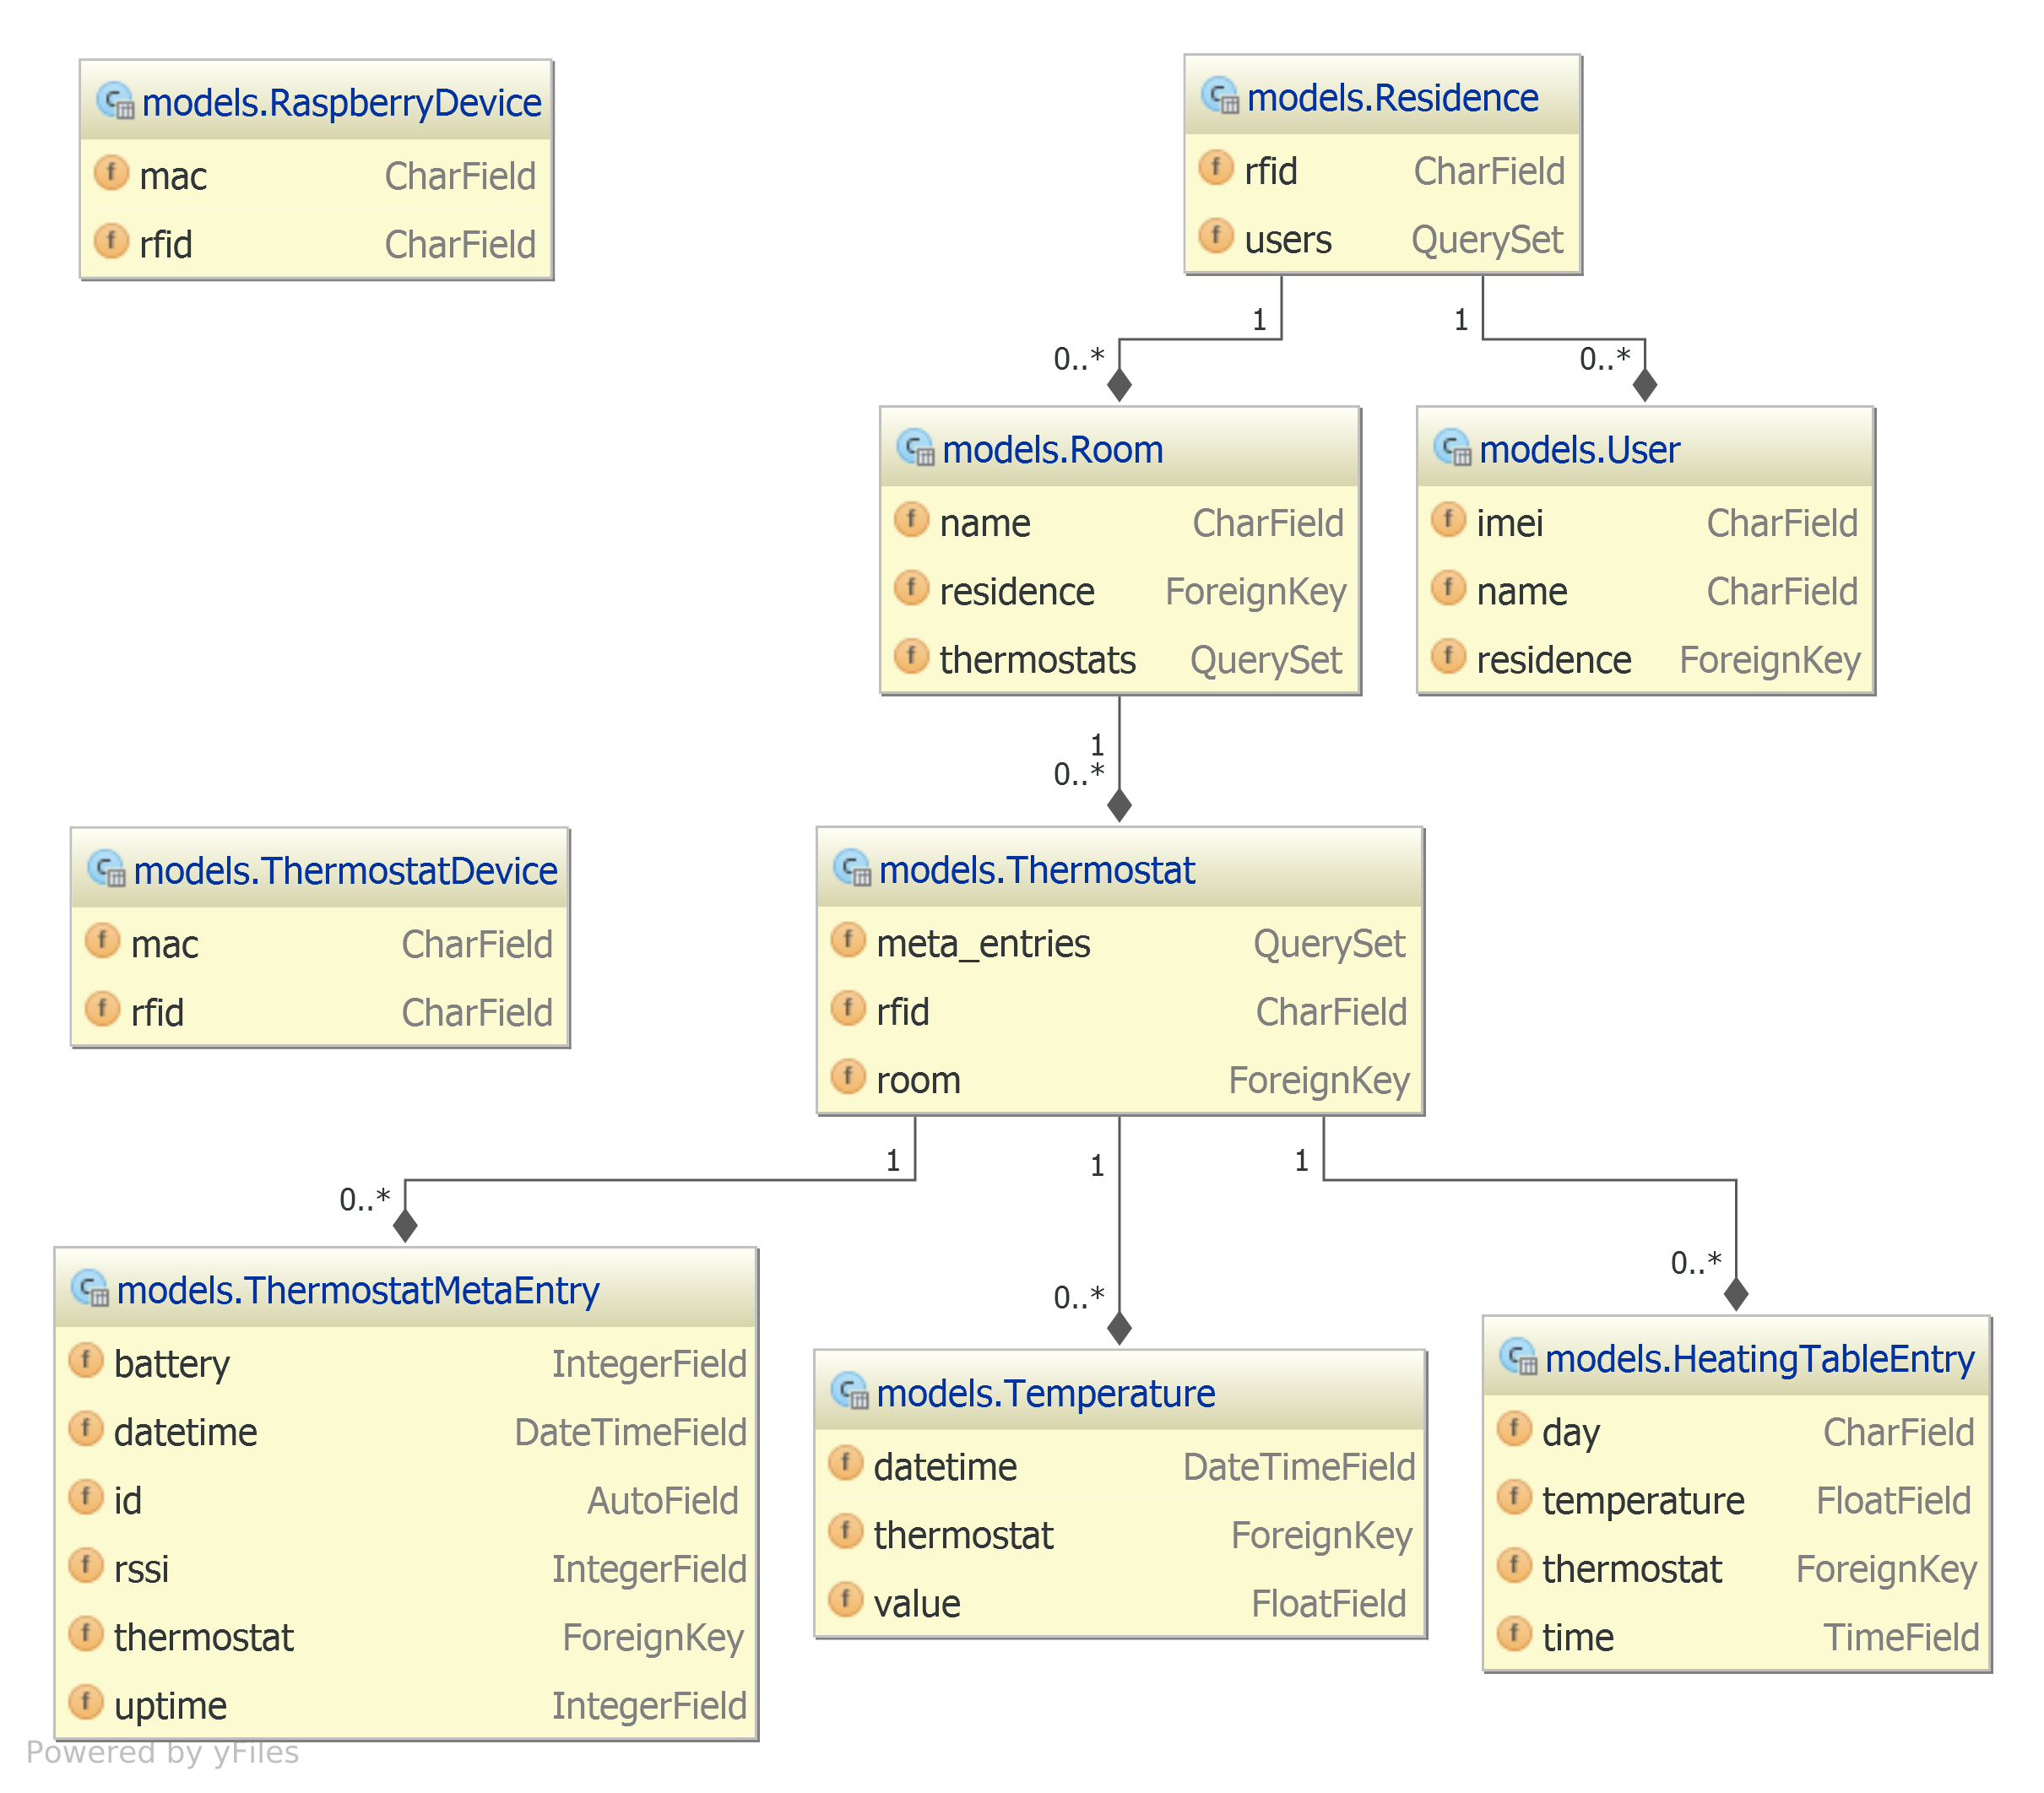
\includegraphics[width=0.8\textwidth]{images/uml_class_diagram_pycharm_highres.png}
\end{center}
\caption{UML class diagram of the models.\todo[inline]{Fix diagram: add all or remove all Querysets. Decide whether or not to display unique constraints.}}
\label{fig:class_diagram}
\end{figure}

Thermostats are organized within rooms and belong to a residence. See Figure~\ref{fig:class_diagram} for a graphical representation of the used models.

\paragraph{Residence}

is identified by the radio frequency identification (RFID) tag number on the deployed local communication gateway. A residence combines users and rooms with their associated thermostats and data into a single encapsulated unit.

\paragraph{User}

is identified by the smart phone's serial number\footnote{The International Mobile Equipment Identity (IMEI), a 15-digit serial number associated to each cell phone, is used to identify each user} and can be registered to at most one residence. 

Room, Thermostat, Temperature, Heating Table Entry, Meta Entry

% temperatures and other data from the local deployment as also the heating schedule from the mobile app.



\subsubsection{Serializers}

\subsubsection{Views}

\subsubsection{Routers}



\subsection{Automated Testing}

Automated software testing is an important part of this project. Django and also the Django REST Framework facilitate automatic testing by providing several classes and tools helping to write and execute tests. Automatic software testing allows the application of test-driven development practices to ensure high software quality.

Furthermore the usage of an Continuous Integration service like Travis CI\footnote{\url{https://travis-ci.org/}} ensures the periodic execution of all tests and logging of the test results.

\subsubsection{Practically Oriented Documentation}

\todo{Screenshot of github.com/spiegelm/smart-heating-server}

\section{Local Deployment}
\label{sec:local_infrastructure}

The local deployments consists of the residential communication gateway and the deployed thermostats with their wireless adapters. The communication gateway collects the data read from the thermostats and sends it to a remote web server. The thermostats are programmable and allow us to modify their behaviour by replacing and adapting the flashed firmware. This project uses the work of previous lab projects as a basis to build upon. The primary focus is to improve the basic functionality of the communication gateway and create an unified but loosely coupled infrastructure by using the RESTful API provided by the server.
See also Figure~\ref{fig:residence_layout} for an overview of the local deployment.

\begin{figure}[h]
\begin{center}
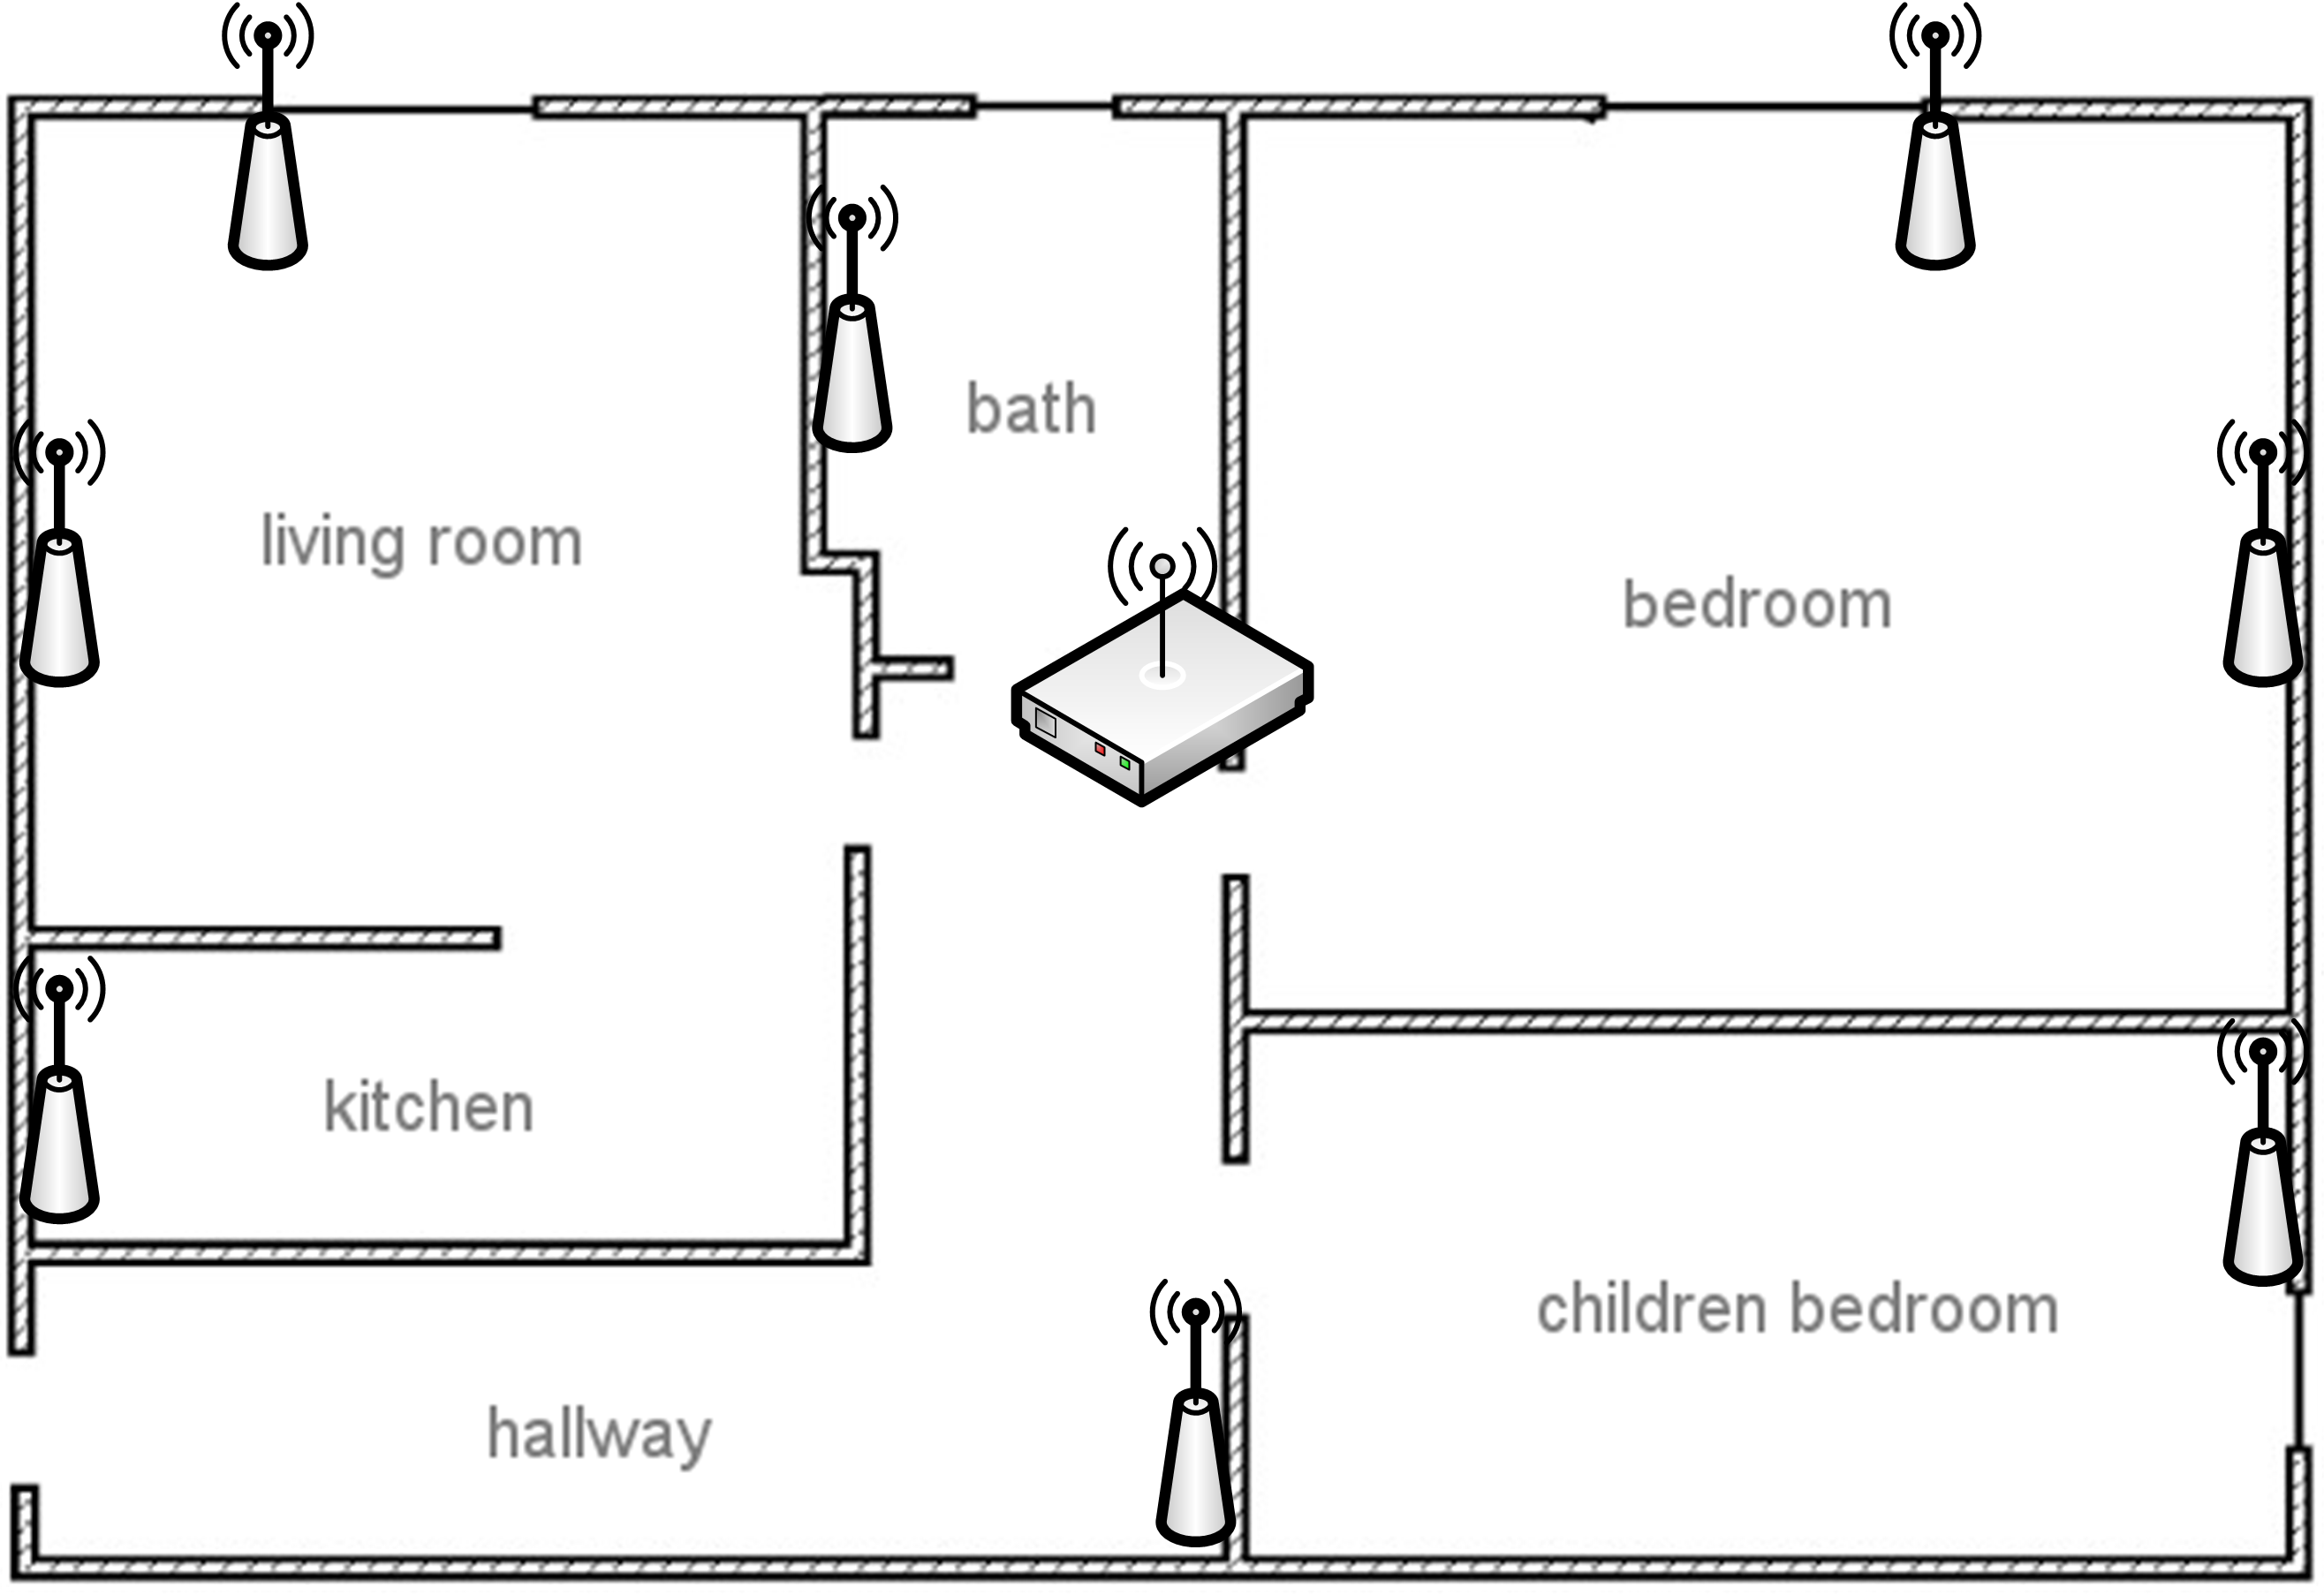
\includegraphics[width=0.8\textwidth]{images/residence_layout_schema.png}
\end{center}
\caption{Example of a residence layout depicting a possible deployment. The local communication gateway is installed in the hallway, connected to the internet and has wireless connections to the deployed thermostats represented as antennas. Source of the original image: \url{http://www.haus-topplicht.de/wp-content/uploads/2013/12/planwohnung2.jpg}}
\label{fig:residence_layout}
\end{figure}

\subsection{Existing Infrastructure}

This lab project builds upon work previously done at the Distributed System Group\footnote{\url{https://www.vs.inf.ethz.ch/}}. 

\subsubsection*{Hardware}

Thermostats, etc

\subsubsection*{Software}

Willis Scripts

\subsection{Design Goals}

Simple, Reliable, Failure resistant

\subsection{Platform and Frameworks}

tunslip6, Python, COAP, aiocoap, requests

\subsection{Implementation}

The communication gateway collects, caches and processes the data read from the thermostats as also the control commands from the server. The local communication gateway works as a proxy server and enables the local deployment to operate independently from the connection to the remote server. This way the last downloaded heating schedule is kept and operated until the server connection is be reestablished. 
%Die grundlegende Einheit jedes Deployments ist die Residence. Eine Residence entspricht genau einem installiertem lokalen System, das die gelesenen Daten der Thermostate sowie Steuerbefehle des Servers sammelt, cached and ausführt. Das lokale Gerät arbeitet als ein lokales Gateway und sorgt dafür, dass der lokale Teil unabhängig von der Verbindung mit dem remote Server funktioniert.
% Temperaturen und andere Meta-Daten von den angebundenen Thermostaten sammelt und cached.

